\documentclass[main.tex]{subfiles}

\pagestyle{fancy}
%\fancyhf{}
\rhead{Assignment 5 - Propeller Analysis}
\lhead{AE4130 | 4738799}
\renewcommand{\headrulewidth}{0.1pt}

\begin{document}

\section{Part 1}
\subsection{Theory}
Blade element momentum theory is a combination of the momentum theory and the blade element theory.
Both of these approaches with their respective simplifications calculate the same quantities like Thrust, Torque etc. Since we have two distinct ways of calculating these quantities an iterative loop can be setup so that we can compute the empirical parameters which reduces the error between these two approaches. The emperical parameters are the induction factor $a$ which calculates the thrust and the azimuthal induction factor $a^{`}$. In the following sections each of these approaches are discussed in more detail
\subsection{Momentum theory}
In this approach we approximate the wind turbine by an actuator disc. Assuming the pressure at station 1 and 4 are the same and there is no discontinuity of velocity as it passes through the infinitely thin actuator disc we can derive the following relation for the thrust for a thin elemental strip of the actuator disc
$$
dF_{x} = \frac{1}{2}  \rho V_{1}^{2}|{4a(1 - a)}|2\pi r dr
$$ 
where
$$ a = \frac{V_{1} - V{2}}{V_{1}}$$
Now if the actuator disc is rotating the torque for the elemental strip is 
$$
dT = 4a'(1 - a)\rho V_{1} \Omega r^{3} \pi dr
$$
where 
$$
a' = \frac{\omega}{2\Omega},  
$$
where
$$
\Omega = angular\;velocity\;of\;the\;blade
$$
$$
\omega = angular\;velocity\;of\;blade\;wake
$$
$$
V_{1} = Velocity\;of\;freestream
$$
$$
F_{x} = The\;thrust\;force
$$
$$
\rho = density\;of\;air
$$
$$
r = radius\;of\;the\;element
$$
\subsection{Blade Element theory}
In this method the wind turbine is no longer assumed to be an actuator disc but is thought of to be made of several sufficiently small blade elements. The primary assumptions of the blade element theory are 
\begin{itemize}
    \item The different blade elements do not interact with each other.
    \item The forces on the blade elements are solely determined by the lift and drag coefficients.
\end{itemize}
The equations of Thrust and Torque for this discretised model are
$$
dF_{x} = \sigma' \pi \rho \frac{V^{2}(1 - a)^2}{\cos{\beta}^2}(C_{L} \sin{\beta} + C_{D} \cos{\beta})rdr
$$

$$
dT = \sigma' \pi \rho \frac{V^{2}(1 - a)^2}{\cos{\beta}^2}(C_{L} \cos{\beta} - C_{D} \sin{\beta})r^{2}dr
$$
where
$$
 \sigma'  = \frac{Bc}{2\pi r}
$$
$$
B = number\;of\;blades
$$
$$
C_{L} = lift\;coefficient\;;of\;the blade\;element
$$
$$
c = chord\;length\;of\;the\;blade\;element
$$
$$
\beta = angle\;between\;the\;resultant\;velocity\;and\;the\;incoming\;flow\;velocity
$$

\begin{figure}[h!]
\vspace*{-0.5em}\centering
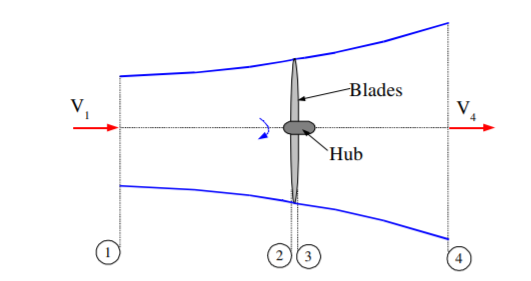
\includegraphics[width=0.6\textwidth]{./Images/Ass5/actdisc}
\caption{Flow around the rotating actuator disc in the momentum model}\vspace*{-0.5em}
\label{fig2}
\end{figure}\vspace*{-1.0em}

\begin{figure}[h!]
\vspace*{-0.5em}\centering
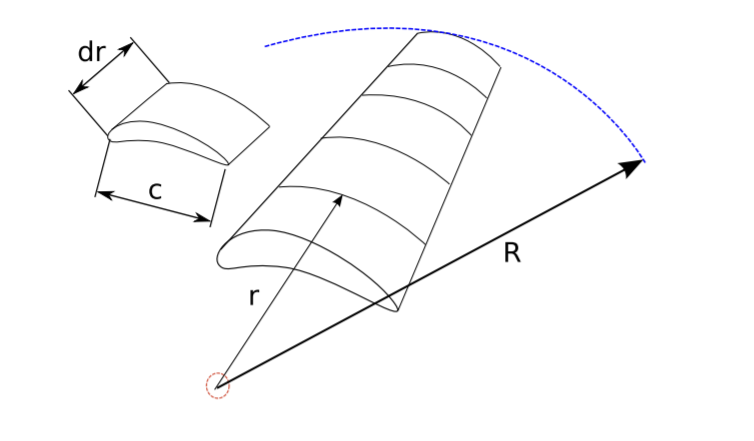
\includegraphics[width=0.6\textwidth]{./Images/Ass5/blade_element_model}
\caption{blade Element Model}\vspace*{-0.5em}
\label{fig2}
\end{figure}\vspace*{-1.0em}

\newpage
\subsection{Velocity Diagram}
\begin{figure}[h!]
\vspace*{-0.5em}\centering
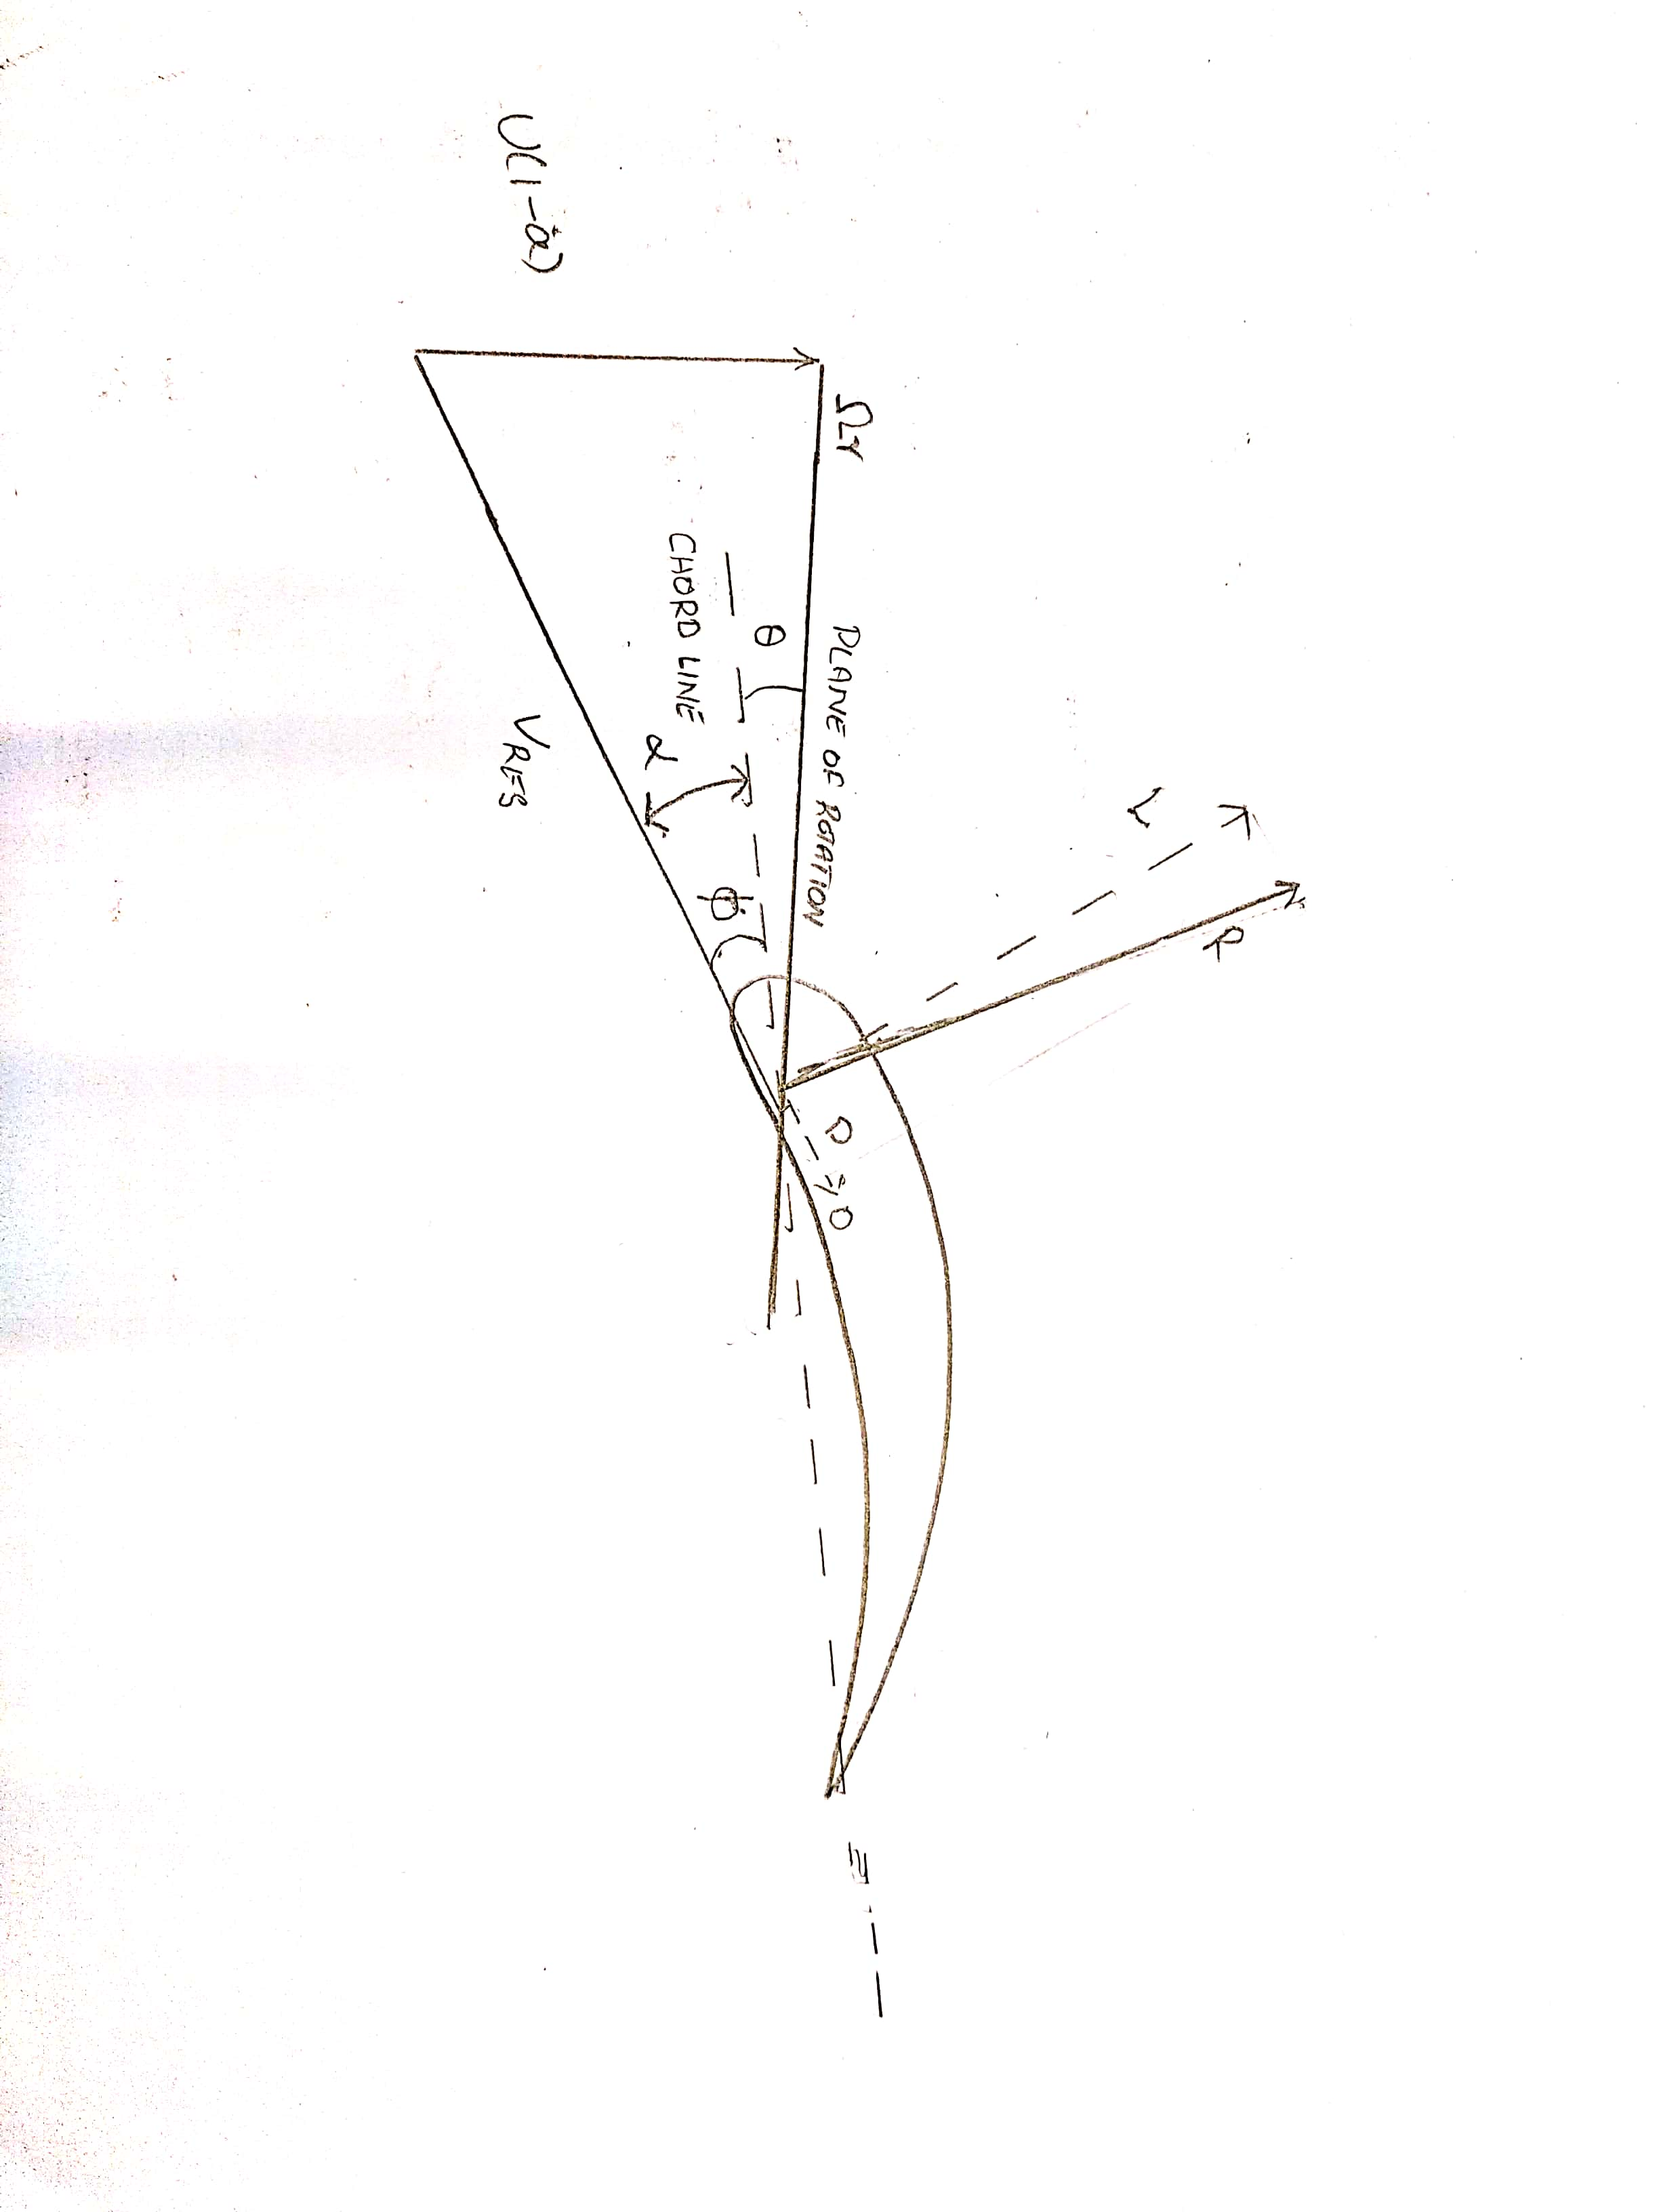
\includegraphics[angle=90,width=0.8\textwidth]{./Images/Ass5/VelocityTriangle}
\caption{Velocity triangle of blade element}\vspace*{-0.5em}
\label{fig3}
\end{figure}\vspace*{-1.0em}
In Figure\ref{fig3} the velocity triangle for a blade element is shown. Here $\phi$ is the inflow angle $\theta$ is the pitch angle $\alpha$ is the angle of attack. 
As can be seen from the figure 
$ \alpha + \theta = \phi$. The incoming velocity near the blade element is $V(1 - a)$ where V is the freestream velocity in the absence of the propeller. This follows from the definition of the induction factor $a$. $V_{RES}$,$R$,$L$ and $D$
are the net resultant velocity, net force on the element, lift and drag forces on the blade element respectively.
\subsection{Definitions}
In this section we introduce the various terms that characterize a propellers performance
\subsubsection{Advance Ratio}
The advance ratio is the ratio of the Velocity of freestream to the velocity of the tip of the propeller.
$$
J = \frac{V}{ND}
$$
Here $V = freestream\;velocity$
$N = rotation\;speed\;in\;revolutions\;per\;second$ and $D = diameter\;of\;the\;propeller$
\subsubsection{Coefficient of thrust}
The thrust coefficient is defined as 
$$
C_T = \frac{T}{\rho N^{2}D^{4}}
$$
where $T$ corresponds to the total thrust.
\subsubsection{Coefficient of Power}
The power coefficient is defined as 
$$
C_P = \frac{P}{\rho N^{3}D^{5}}
$$
where $P$ corresponds to the total power.
\subsubsection{efficiency}
The efficiency is the ratio of the power that can be extracted due to the thrust and the power required by the propeller.
$$
\eta = \frac{TV}{P} =\frac{C_{T}J}{C_{P}}
$$
\subsection{Prandtl tip loss factor}
Similar to wing tip vortices
\subsection{Radial flow correction for propellers}
One of the many simplification of BEM is that there are an infinite number of blades or the rotor. When we encounter a discontinuity like the tips errors are introduced in the BEM Analysis. The tip induces circulation into the wake leading to losses and interaction of the vortices with the propeller itself.
\newpage
\begin{figure}[h!]
\vspace*{-0.5em}\centering
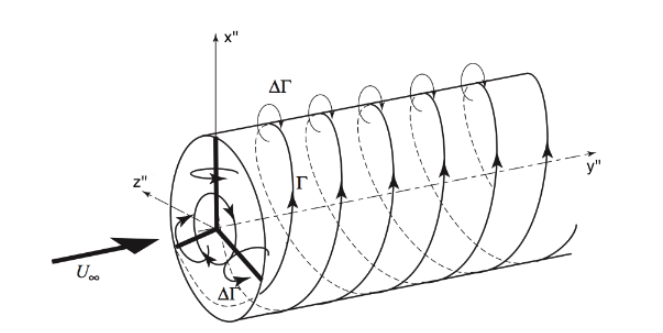
\includegraphics[,width=0.5\textwidth]{./Images/Ass5/wingtipvortices}
\caption{Circulation in the wake of the propeller}\vspace*{-0.5em}
\label{fig4}
\end{figure}\vspace*{-1.0em}
$$
Q = \frac{2}{\pi}\cos^{-1}{\exp({\frac{B}{2}\frac{1 - r}{r\sin{\phi}}}})
$$
\subsection{Radial flow correction for propellers}
The BEM models do not incorporate the reymolds scaling effects inherently[cite]. BEM fundamentally assumes a quasi 2D flow with no iteraction between the blade elements. Locally separation regions of the blade elements have a higher radial gradient compared to a chordwise gradient. This results in a net flow of the fluid which in turn requires additional energy from the rotor. Semi emperical corrections were proposed by [cie Snel etal]. Near the tip due to a lower angle of attack theis radial flow is reduced. The centrifugal pumping correction is then applied from the root to 85 percent of the blade
$$
C_{N_{3D}} = C_{N_{2D}} + 1.5(\frac{c}{r})^2 + (C_{L,pot} - C_{N_{2D}})(\frac{\omega r}{V_{l}})^2
$$
where
$V_{l}$ = velocity across the propeller,

$C_{N_{2D}}$ = Uncorrected 2D normal force,
$C_{L,pot}$ =Lift from potential flow theory

$C_{N_{3D}}$ = Corrected normal force 


\section{Part 2}
\subsection{JAVAPROP}
JAVAPROP as the name suggest is a JAVA based propeller analysis software which uses the BEM algorithm. The experimental data for the propeller has been taken from\cite{UIUC}. A propeller of diameter 9 inch with a pitch of 6 inch per revolution was chosen for the current study. The airfoil section was chosen as a flat plate at an angle of attack 5.8 was chosen (default setting in JAVAPROP) as there was no section specified. Since the geometry data was specified from $\frac{r}{R} = 0.15$ we can assume that the hub is upto that distance.
 


\section{Results of BEM Analysis}
For this part of the assignment, JAVAProp is used to analyze the propeller. JAVAProp also uses BEM theory to design and analyze propellers. Since the wind-tunnel database already contained the detailed geometry details of the blade, the direct design feature of JAVAProp has been exploited for the analysis. The wind-tunnel results of the 9x4" Free Flight propeller were obtained from the UIUC Propeller Data Site\cite{UIUC} by Prof. Deters\cite{deters2014reynolds}\cite{deters2014performance}.\\
\newline The propeller has been modelled in JAVAProp and its performance characteristics have been compared with the experimental data(for one blade angle setting as mentioned). Later, a moderate and constant Thrust of 65N is used to study the axial velocity increase across the span of the blade. Further, for a fixed power setting of 0.08kW the effect of blade number, propeller diameter and blade aspect ratio are also analyzed. The geometry information of the chosen propeller is provided in Figure \ref{fig4}.\\
\newline The results have been compared and studied for an angle of attack of approx. 5.8$^{\circ}$ for all four airfoil sections. Due to unavailability of airfoil data, the flat plate Reynolds number of 100000 is chosen in JAVAProp. Other analysis details are provided in each subsection wherever necessary.

\begin{figure}[h!]
    \centering
    \vspace{-1em}
    \subfloat[Blade Front View]{
        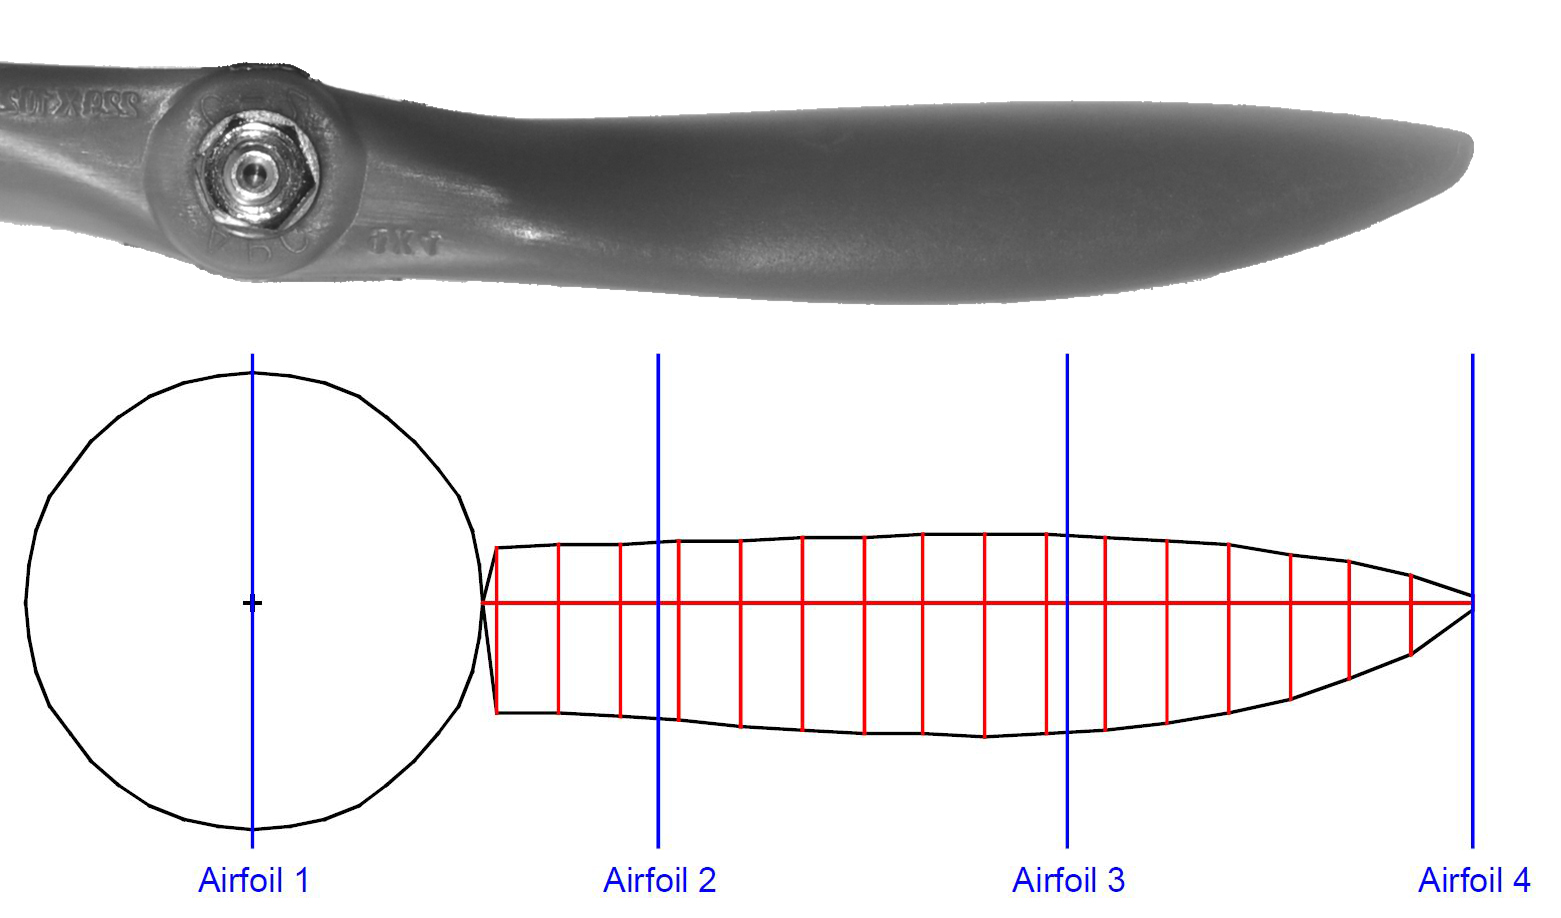
\includegraphics[width=0.55\textwidth] {./Images/Ass5/BladeShape}
        \label{fig4a} }
    \subfloat[Blade geometry details from \cite{UIUC}]{
         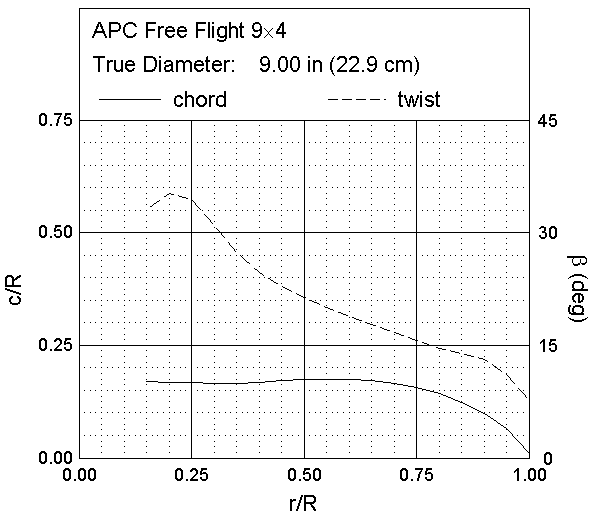
\includegraphics[width=0.37\textwidth] {./Images/Ass5/apcff_9x4_geom}
        \label{fig4b} }\\
    \caption{Chosen blade geometry details}
    \label{fig4}
\end{figure}

\vspace{1cm}
\subsection{Performance Characteristics Comparison}
Figure \ref{fig5} shows the results from the comparative study between the experimental(wind tunnel) and JAVAProp analysis. The settings mentioned in Table \ref{table1} were used for the \textit{Multi-analysis} in JAVAProp.

\begin{table}[h!]\begin{center}\begin{tabular}{ c c } 
 \hline \rowcolor{lightgray}
  \hspace{0.5cm}Physical Quantity\hspace{0.5cm} & \hspace{0.5cm}Value\hspace{0.5cm} \\
  \hline
  No. of Blades & 2\\
 \hline
  RPM & \{3014,4033,5049,6057\}\\
 \hline
  Prop. Diameter & 0.2286m\\ 
   \hline
 Spinner Dia. & 0.03429m \\ 
\hline
Velocity & 5.7ms$^{-1}$ \\ 
\hline
Power & 65W \\ 
\hline
Re & 100000 \\ 
\hline
\end{tabular}\caption{JAVAProp Setup}\vspace*{-2em}\label{table1}\end{center}\end{table}


\begin{figure}[h]
    \centering
    \vspace{-1.4em}
    \subfloat[RPM = 3014]{
        \hspace{-2cm}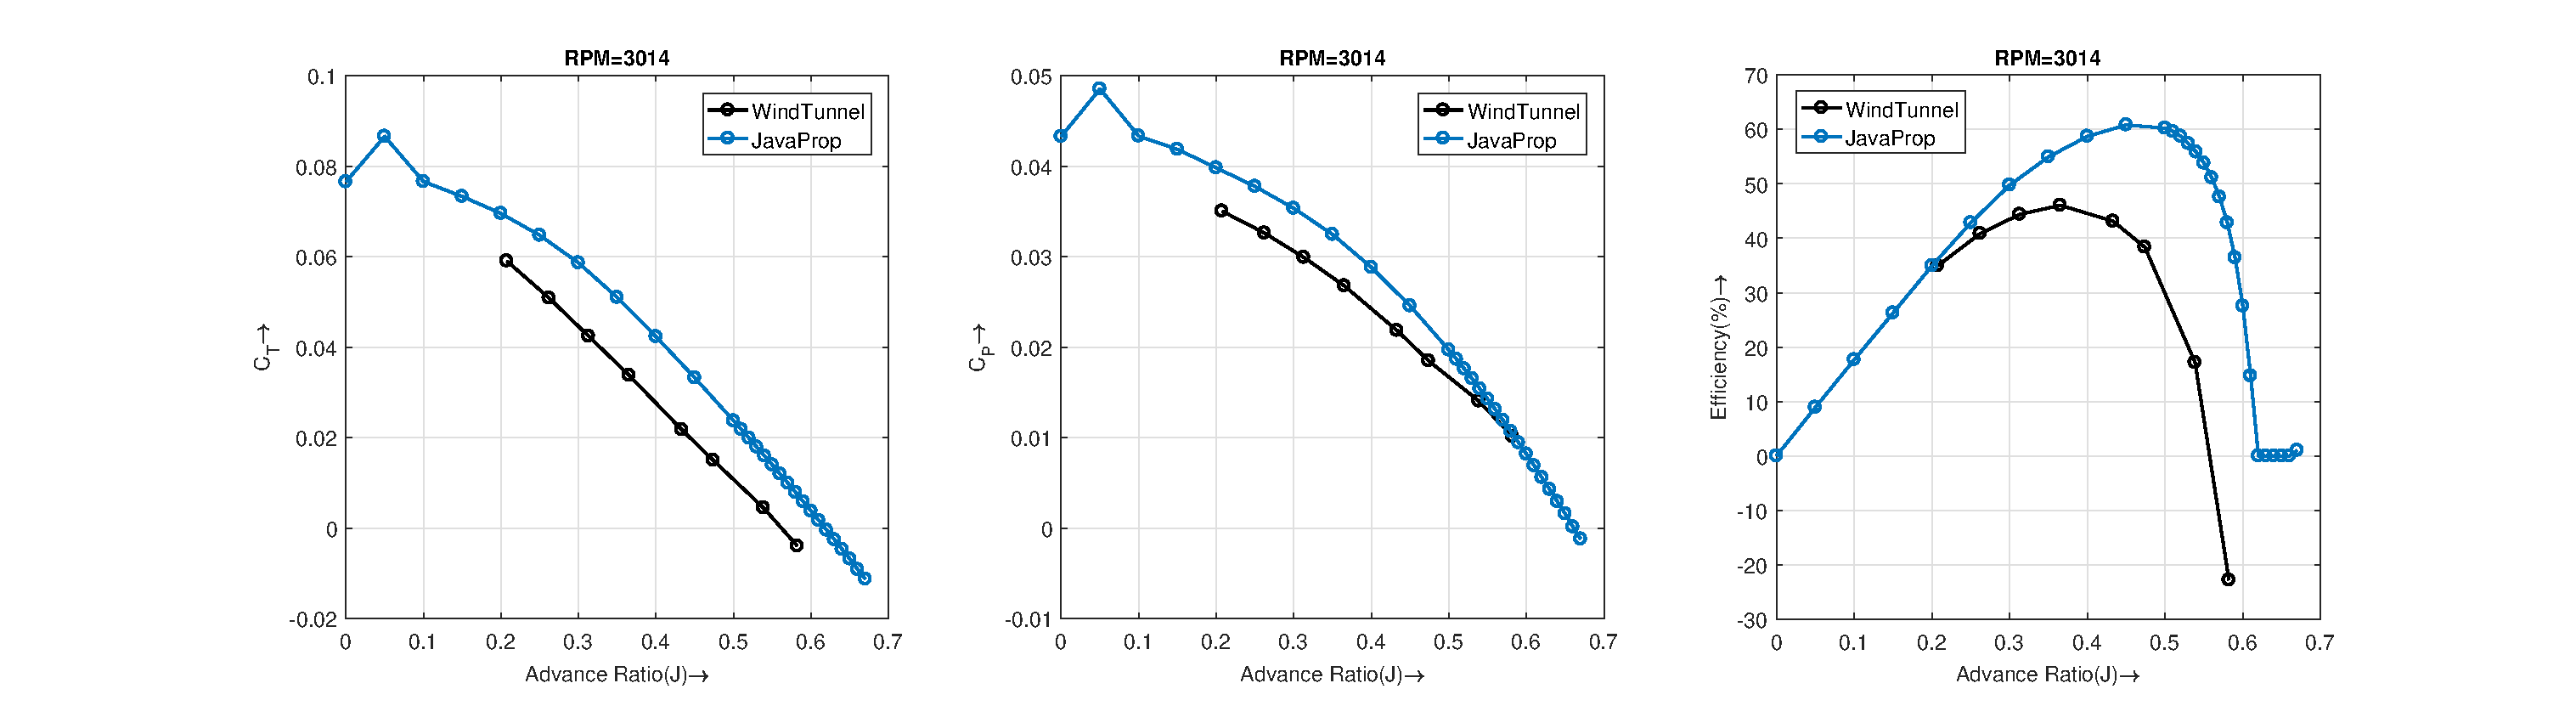
\includegraphics[width=1.2\textwidth] {./Images/Ass5/PerfComparison3014}
        \label{fig5a} }\vspace{-1.2em} \\ 
    \subfloat[RPM = 4033]{
         \hspace{-2cm}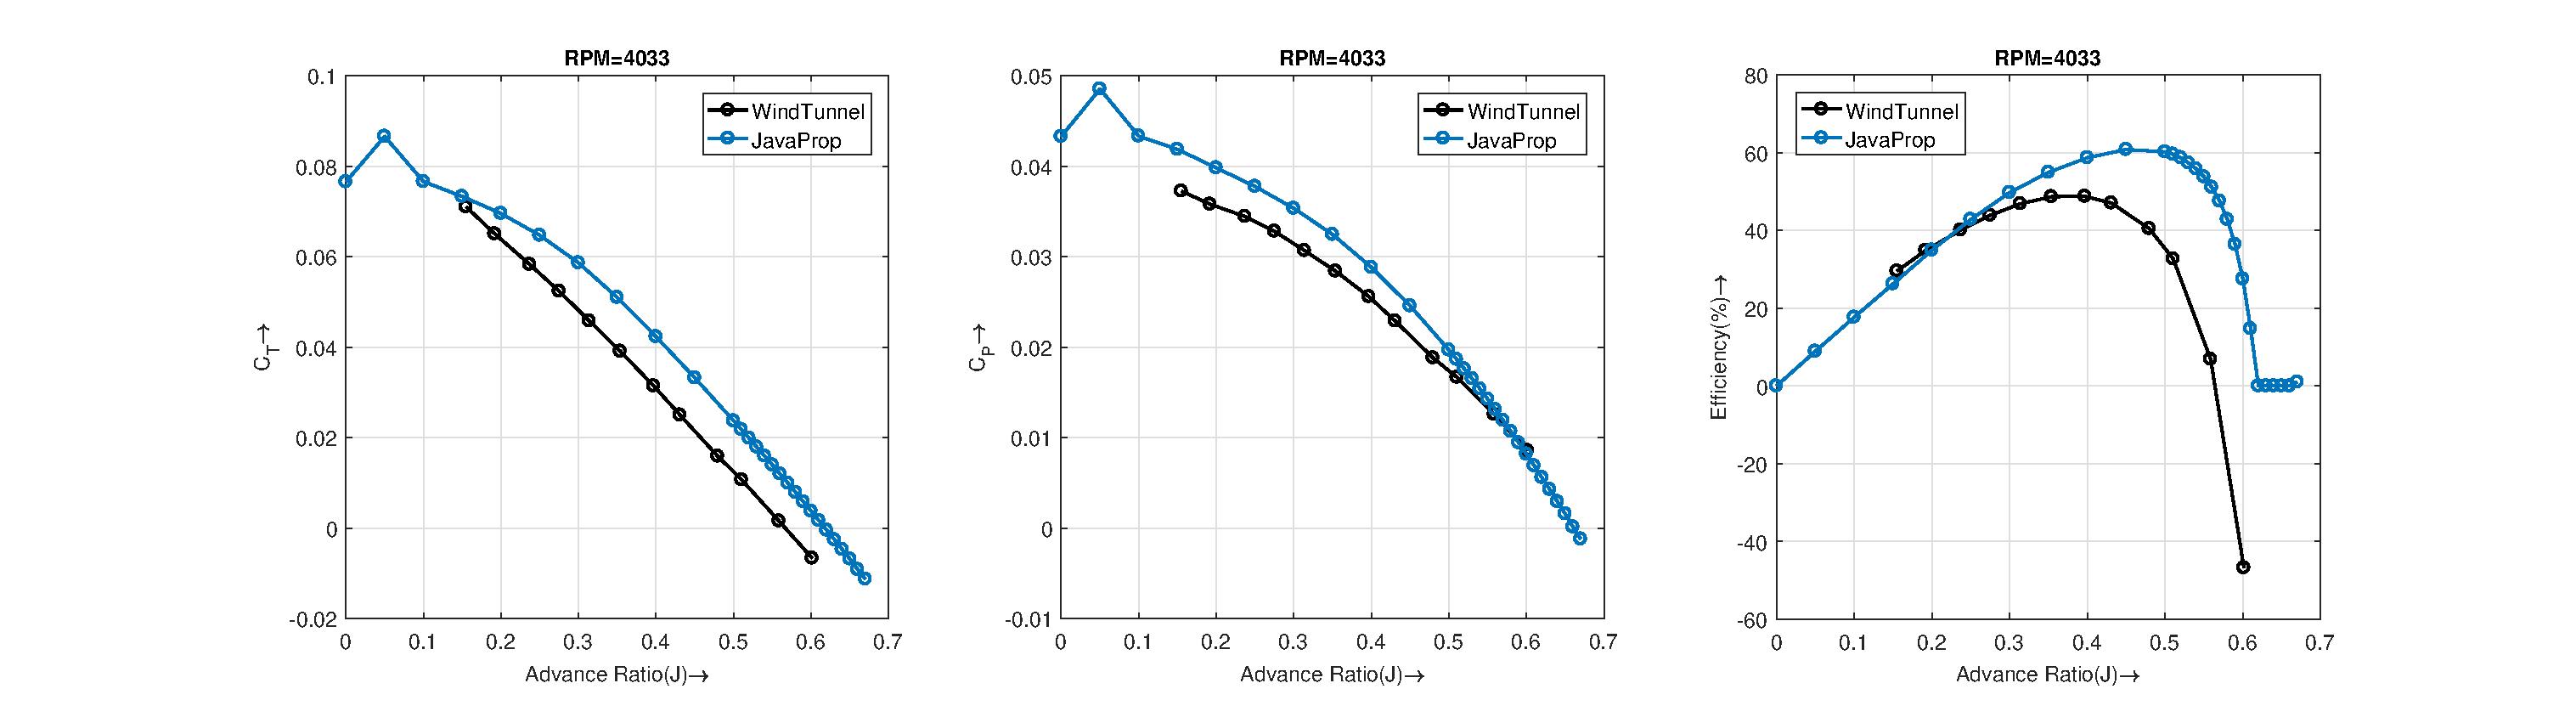
\includegraphics[width=1.2\textwidth] {./Images/Ass5/PerfComparison4033}
        \label{fig5b} }\vspace{-1.2em} \\
    \subfloat[RPM = 5049]{
        \hspace{-2cm}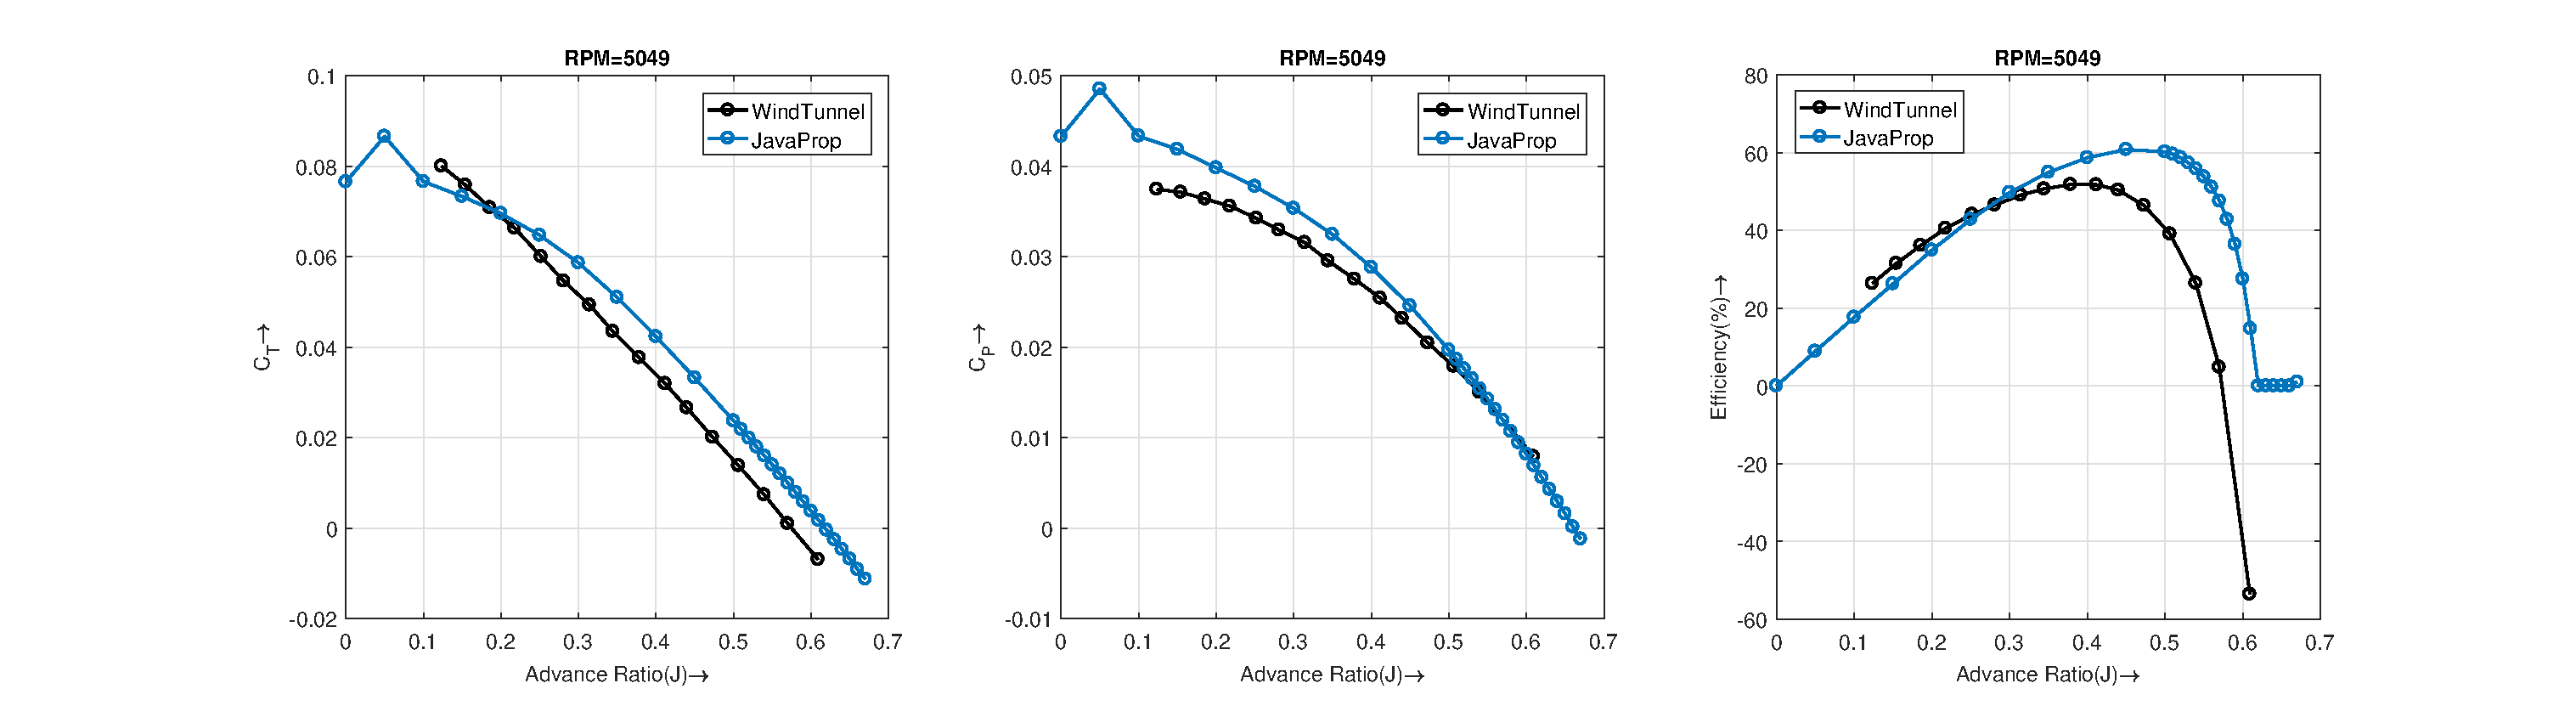
\includegraphics[width=1.2\textwidth] {./Images/Ass5/PerfComparison5049}
        \label{fig5c} }\vspace{-1.2em} \\ 
    \subfloat[RPM = 6057]{
         \hspace{-2cm}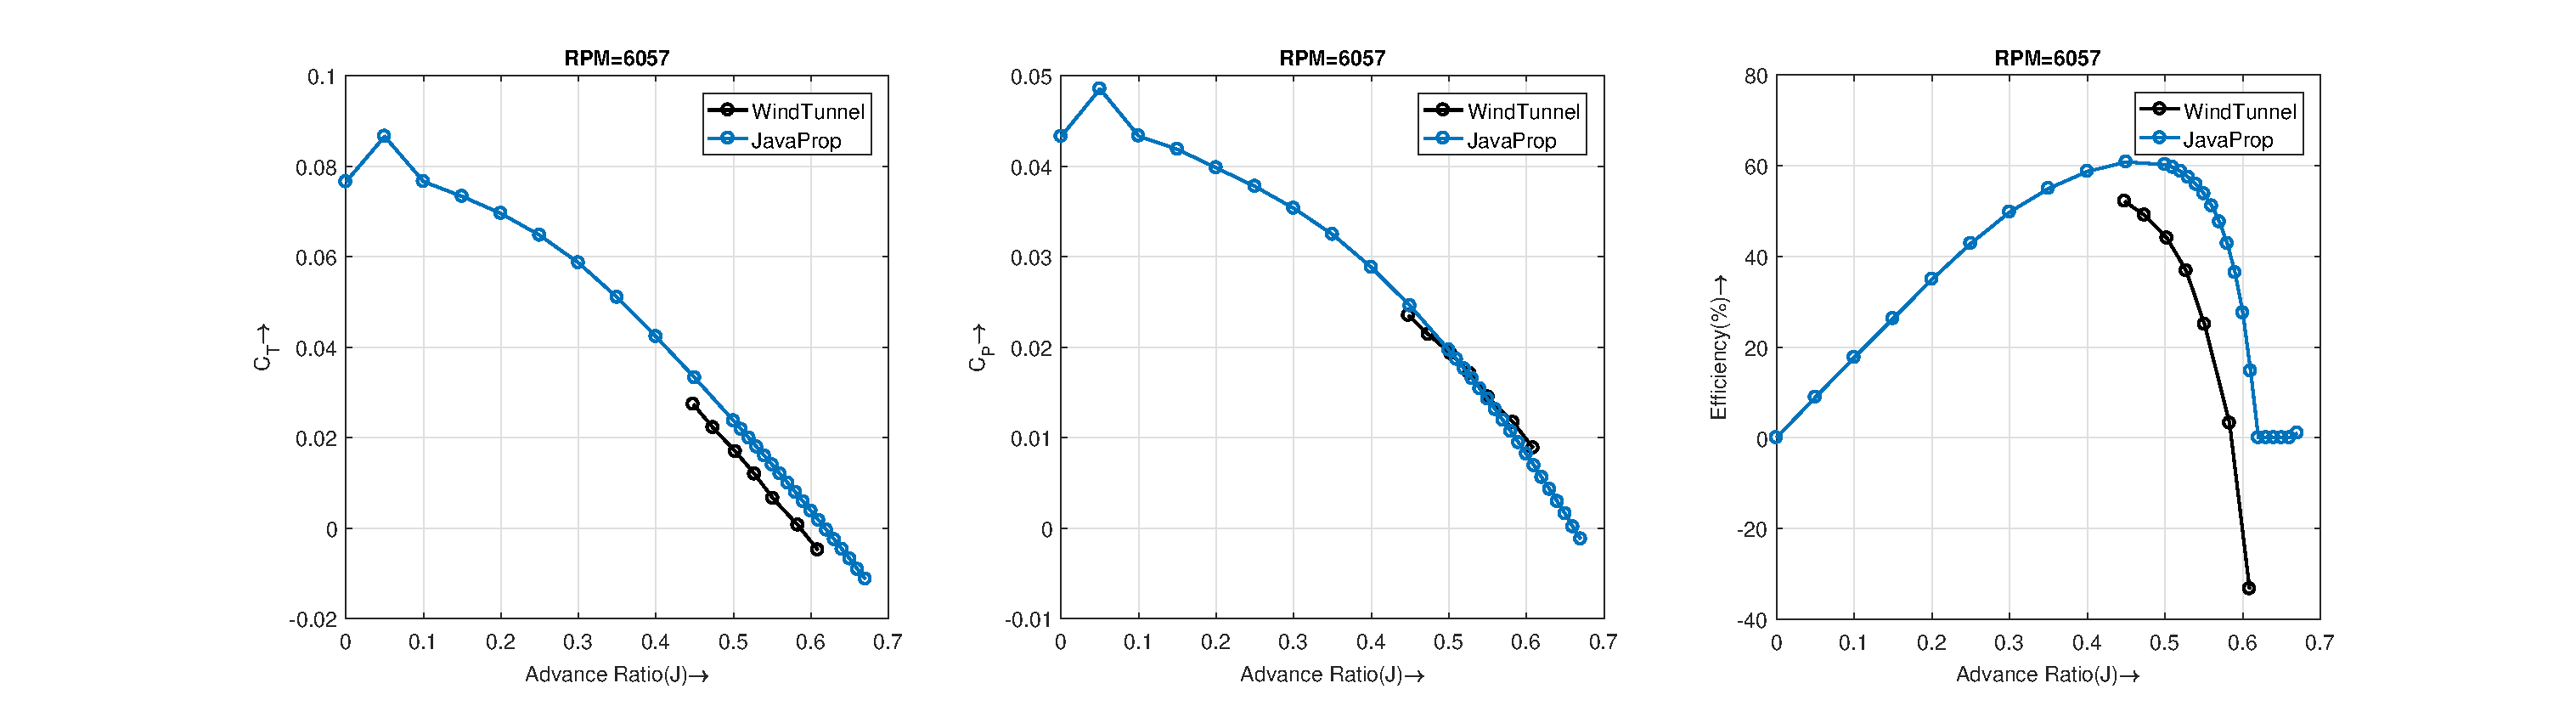
\includegraphics[width=1.2\textwidth] {./Images/Ass5/PerfComparison6057}
        \label{fig5d} }\vspace{-1.2em} \\
    \caption{Performance Comparison}
    \label{fig5}
\end{figure}

\newpage
\printbibliography[title={References}]
\end{document}
